We wish to use random graphs to test vertex classifiers. An issue that arises is that the generative
models presented so far do not suggest any natural labeling for the vertices of the resultant graphs.
Thus, we propose some models for generating labeled small-world and scale-free networks with a natural community structure.

\begin{definition}
  A \textbf{labeled graph} is a graph $G$ and a function $c : V_G \to S$, where $S$ is an arbitrary.
  For $u \in V_G$, we call $c(u)$ the \textbf{class} of $u$.
\end{definition}

In considering labeled graphs, it is useful to look at not only at each vertex's degree, but also the
number of neighbors with the same label vs the number of neighbors with a different label. For
convenience, we define these quantities as follows:

\begin{definition}
  Let $G$ be a labeled graph, $u \in V_G$. The \textbf{same-class degree} of $u$, $\deg_{\textit{same}}(u)$, is
  the number of vertices in the neighborhood of $u$ in the same class as $u$. Similarly, $\deg_{\textit{diff}}(u) =
  \deg(u) - \deg_{\textit{same}}(u)$ is the number of vertices in a different class.
\end{definition}


\section{Noisy Complete Components (NCC) Graphs}

\begin{definition}
  Let $m$ be a natural number. We construct the \textbf{complete components
    graph} of order $n = 2m$ as follows. Let $V = \{1,2, ..., 2m\}$, and then define
  $E$ by

  \[
    E = \{ (u,v) : u,v \in \{1,...,m\} ~\text{or}~ u,v \in \{m+1,...,2m\} \}
  \]

  i.e. the disjoint union of two complete graphs of order $m$. In addition, we label the graph by the
  function

  \[c(u) =
      \begin{cases}
        0 &: u \in \{1,...,m\} \\
        1 &: u \in \{m+1,...,2m\}
      \end{cases}
    \]
\end{definition}

\begin{definition}
  \label{def:ncc}
  Let parameters $(m,p,q)$ be given, $m \in \mathbb{N}$ and $p,q \in [0,1]$, and let $G_0$ be the
  complete components graph of order $2m$. We construct a \textbf{Noisy Complete Components (NCC)}
  graphs as follows.

  Iterate over ever pair of vertices in the graph (i.e. the edge set of
  $K_{2m}$). For every pair $(u,v) \in E_{G_0}$, that is, for the edges that
  already exist in $G_0$, we delete the edge with probability $q$. Likewise, for
  each pair $(u,v) \notin E_{G_0}$, we add the edge $(u,v)$ with probability
  $p$.

  The resultant graph is an NCC graph. This definition generalizes easily 
  to graphs with multiple components, and components with different sizes, 
  but the defined graph will be sufficient for our purposes.
\end{definition}

We will now inspect the properties of such graphs in order to demonstrate that they are, in fact,
small worlds graphs in the subset of the parameter space in which we're interested. Before doing so,
we recall some basic distributions from statistics

\begin{definition}
  A \textbf{Bernoulli distribution} with probability $p$ is a discrete probability distribution
  with probability mass function

  \[
    f(x) =
      \begin{cases}
        p &:~ x = 1 \\
        1-p &:~ x = 0 \\
        0 &:~ \text{otherwise}
      \end{cases}
    \]

  A \textbf{binomial distribution} of $n$ trials with probability $p$, denoted $B(n,p)$ is equal to
  the sum of $n$ independent bernoulli random variables with probability $p$. Its probability mass
  function is

  \[
    f(x) = {n \choose x} p^x(1-p)^{n-x}
  \]

  for $x = 0,1,...,n$ and $0$ outside that range.

  For a more complete discussion of these distributions and the probabilitity theory employed in
  this chapter, see ~\cite{CaseBerg:01}.
\end{definition}


\begin{theorem}
  \label{thm:ncc_deg}
  Let $G$ be an $(m,p,q)$ NCC graph and $u$ a vertex in $G$. Then $\deg(u)$ follows the distribution
  $X + Y$, where $X$ and $Y$ are (independent) binomial random variables, $X \sim B(m-1,1-q)$ and
  $Y \sim B(m,p)$. Moreover, $\deg_{\textit{same}}(u) = X$ and $\deg_{\textit{diff}}(u) = Y$.
\end{theorem}
\begin{proof}
  First, observe that adding and deleting edges to an NCC graph is done independently for each edge.
  In other words, the existence or nonexistence of any edge of $G$ is independent of every other edge.
  In addition, the number of edges added between $u$ and all other different-class vertices is equal
  to a sum of $m$ Bernoulli random variables of probability $p$, because there are $m$ possible edges
  from $u$ to the opposite class. Thus $deg_{diff}(u)$ follows a binomial distribution on $m$ trials,
  $deg_{diff}(u) = Y \sim B(m,p)$.

  In the case of same-class edges, we will consider the probability that an edge is \textit{preserved}
  rather than deleted. Edges are preserved with probability $(1-q)$, so as in the different-class
  case, we can see that the same-class degree of $u$ follows a binomial distribution on $(m-1)$
  trials, $deg_{same} = X \sim B(m-1,1-q)$.

  As we've counted both the same- and different-class degrees, it is clear that $deg(u) = X + Y$.
\end{proof}

We must take care to note that this is not the same thing as the degree distribution over the whole
graph $G$. While each edge with respect to a single vertex is picked independently, this is not true
over the whole graph, since each edge is connected to two vertices.

\begin{remark}
  The previous theorem shows that the following is true
  \begin{enumerate}
  \item $\E(\deg_{\textit{same}}(u)) = (m-1)(1-q)$ and $\E(\deg_{\textit{diff}}(u)) = mp$, where $\E$ is expectation.
  \item $\Var(\deg_{\textit{same}}(u)) = (m-1)(1-q)q$ and $\Var(\deg_{\textit{diff}}(u)) = mp(1-p)$, where $\Var$ is
    variance.
  \item $\E(\deg(u)) = (m-1)(1-q) + mp$ by linearity of expectation.
  \item $\Var(\deg(u)) = (m-1)(1-q)q + mp(1-p)$ by linearity of variance on independent random
    variables.
  \end{enumerate}
\end{remark}

% \begin{theorem}
%   Let $u$ and $v$ be vertices in an $(m,p,q)$ NCC graph. We write $P(\spd(u,v) = k)$ for the probability
%   that the shortest path between $u$ and $v$ is equal to $k$.

%   If $c(u) = c(v)$, then $\E(P(\spd(u,v) = 1)) = 1-q$ and
%   $\E(P(\spd(u,v) = 2)) = 1- (1 - (1-q)^2)^{m-1} (1-p^2)^{m}$.

%   If $c(u) \neq c(v)$, then $\E(P(\spd(u,v) = 1)) = mp$ and
%   $\E(P(\spd(u,v) = 2)) = 1- ((1-q)(1-p) + q)^{m-1}(pq+(1-p))^n$.
% \end{theorem}
% \begin{proof}
%   For the cases where $\spd(u,v) = 1$, the results follow immediately from definition \ref{def:ncc}.

%   \textbf{Note to Professors:} while typing this, I found an error. I need to nudge around the random
%   variables in the probability formulas because I'm operating under the assumption that 1) there's an
%   edge between $u$ and each neighbor, and 2) there's not an edge between $u$ and $v$. This just
%   reduces the number of trials on the binomial variables so it should just be changes by factors of $p$
%   and $q$, but I didn't have time to work it out.

%   % TODO: fix this. X changes slightly because we assume that the trial between u and v failed, and
%   % the trial between u and each neighbor succeeded.
%   Now, we consider the case where $\spd(u,v) = 2$ and $c(u) = c(v)$. Under these circumstances, we
%   denote the number of same-class neighbors by the random variable $X$ and the number of
%   different-class neighbors by $Y$. A length-2 path between $u$ and $v$ must exist unless we fail to
%   preserve/add every single edge from the neighborhood of $u$ to $v$, which happens with probability
%   $q^X(1-p)^Y$. Thus $P(\spd(u,v) = 2) = 1 - q^X(1-p)^Y$.

%   Since $X$ and $Y$ are binomial random variables by theorem \ref{thm:ncc_deg}, their probability mass
%   functions are:

%   \begin{align*}
%     f_X(x) &= {n-1 \choose x} (1-q)^xq^{n-1-x} \\
%     f_Y(y) &= {n \choose y} p^y(1-p)^{n-y}
%   \end{align*}

%   using the expectation formula, we can compute $q^x$ and $p^Y$:

%   \begin{align*}
%     \E(q^X) &= \sum_{i=0}^{n-1}q^i{n-1 \choose i}(1-q)^iq^{n-1-i} \\
%             &= q^{n-1}\sum_{i=0}^{n-1}{n-1 \choose i}(1-q)^i(1)^{n-1-i} \\
%             &= q^{n-1}(2-q)^{n-1} \\
%             &= (1 - (1 - q)^2)^{n-1}
%   \end{align*}

%   \begin{align*}
%     \E((1-p)^Y) &= \sum_{i=0}^{n}(1-p)^i{n \choose i}(1-(1-p))^i(1-p)^{n-i} \\
%             &= (1-p)^{n}\sum_{i=0}^{n}{n \choose i}(1-(1-p))^i(1)^{n-i} \\
%             &= (1-p)^{n}(p-1))^{n} \\
%             &= (1 - p^2)^{n}
%   \end{align*}
%   thus, in this case,

%   \[ P(\spd(u,v) = 2) = 1 - (1 - (1-q)^2)^{n-1}(1-p^2)^n \]

%   % TODO: fix this. Y changes slightly because we assume that the trial between u and v failed.
%   In the case where $c(u) \neq c(v)$, the probability becomes $P(\spd(u,v) = 2) = 1 - q^Y(1-p)^X$, so
%   by an analogous computation, we get

%   \[ P(\spd(u,v) = 2) = 1 - (q + (1-p)(1-q))^{n-1}(pq + (1-p))^n \]
% \end{proof}


These graphs are extremely regular, so they do not exhibit scale-free properties. Thus, we
also propose a variant on the Barab\'asi-Albert model which adds labels while preserving the power
law degree distribution.

%% prove theorem: the following are equal: frobenius norm of a matrix,
%% \sum{\lambda^2}, number of edges in G (or something like this)

% sketch: recall \sum \lambda_i = \tr(M). Consider A^2, whose trace is the sum
% of degrees

\section{Class-Weighted Barab\'{a}si-Albert (CWBA) Graphs}

% TODO: refer back to previous chapter definition of BA 
\begin{definition}
  Let parameters $G_0$ and $m \leq |G_0|$ be given as in the BA process as well
  as a finite set of labels $S$ and a factor $\rho \ge 1$. In addition, suppose
  each vertex in $G_0$ has been labeled by an element of $S$. Given a graph
  $G_t$, we build $G_{t+1}$ as follows.

  As in the BA process (see Definition \ref{def:ba}, page \pageref{def:ba}), we will add one new vertex and draw
  edges using preferential attachment, however, we label our new vertex $l$, which is chosen from $S$
  with uniform probability. Then, we reweight the probability of drawing each edge in order to favor
  vertices with label $l$ by a factor of $\rho$.

  Define $S_l$ to be the set of vertices with label $l$. Then, we define the
  probability of drawing an edge to a vertex $u$ as

  \[
    p_u = \begin{cases}
      \frac{\rho\deg(u)}{w} &: u \in S_l\\
      
      \frac{\deg(u)}{w} &: u \in (V_G - S_l)\\
    \end{cases}
  \]

  where $w$ is the weighted degree sum,

  \[
    w = \rho \sum_{v \in S_l}\deg(v) + \sum_{v \in (V_G - S_l)}\deg(v)
  \]

  We call this random process the \textbf{class-weighted Barab\'asi-Albert
    (CWBA) process} and we call graphs sampled from this model \textbf{CWBA
    graphs}.

  % TODO: add example
\end{definition}

We do not prove that CWBA graphs are scale-free, but degree plots over arbitrary choices of
parameters suggest that they are. See Figure ~\ref{fig:cwba_degs}.

\begin{figure}[H]
  \centering
  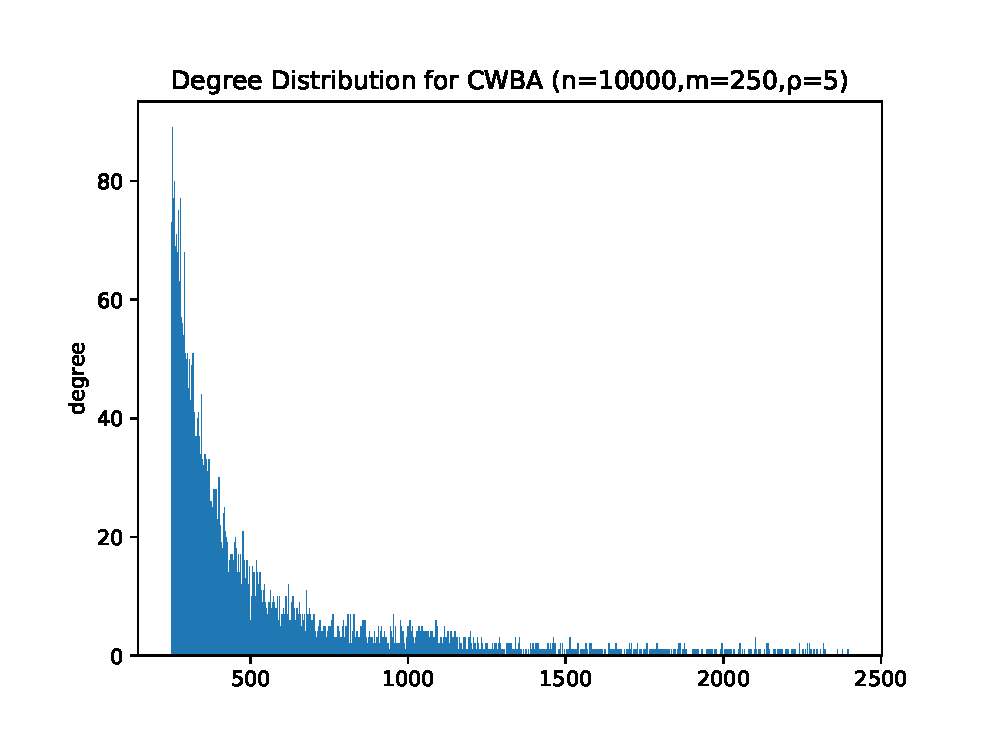
\includegraphics[width=0.7\textwidth]{CWBA_degree_dist.eps}
  \caption{Degree distribution of CWBA graphs demonstrates scale-free behavior.}
  \label{fig:cwba_degs}
\end{figure}

Between the apparent power law degree distribution and the straightforward reweighting of the
preferential attachment algorithm, we expect CWBA graphs to be a reasonably good indicator of how a
metric-based classifier would perform on real-world data.

%%% Local Variables:
%%% mode: latex
%%% TeX-master: "../Main"
%%% End: